\documentclass{article}
\usepackage[utf8]{inputenc}
\usepackage[spanish]{babel}
\usepackage{listings}
\usepackage{graphicx}
\graphicspath{ {images/} }

\begin{document}

\begin{titlepage}
    \begin{center}
        \vspace*{1cm}
            
        \Huge
        \textbf{Informe de implementación}
            
        \vspace{0.5cm}
        \LARGE
        Informática II
            
        \vspace{1.5cm}
            
        \textbf{Juan Pablo Areiza Jiménez\\Santiago Montoya Leal}
            
        \vfill
            
        \vspace{0.8cm}
            
        \Large
        Departamento de Ingeniería Electrónica y Telecomunicaciones\\
        Universidad de Antioquia\\
        Medellín\\
        Septiembre de 2021
            
    \end{center}
\end{titlepage}

\tableofcontents
\newpage
\section{Introducción}\label{intro}
Como iniciativa para la actualización en la forma de presentar las nacionalidades de los competidores que han llegado al podio de triunfadores, para los juegos olímpicos de París 2024, se plantea una implementación tecnológica, la cual permite presentar en una pantalla con leds RGB la nacionalidad de los triunfadores. Para la realización de esta implementación, se utiliza la programación orientada a objetos, con el fin de procesar y muestrear las banderas de cada país según sea el caso, este muestreo se guarda en una estructura de datos tipo byte, lo que ayuda a reducir el uso de memoria, posteriormente, este arreglo se lleva al montaje de la pantalla con leds RGB y en esta, se presenta la bandera muestreada.
\section{Marco teórico} \label{mt}
En el proceso de digitalización de una imagen, se realiza un muestreo de la misma, este puede ser un submuestreo o sobremuestreo de acuerdo con las dimensiones de la imagen y el espacio destinado para la digitalización de esta. Una técnica de muestreo para la digitalización de imágenes, consiste en la realización de un muestreo espacial, en el cual se escogen las muestras representativas, a partir de la especificación de la intensidad o color de la imagen en unos puntos determinados. 


En el muestreo espacial, se divide la imagen en un conjunto de muestras, todas de igual dimensión, posteriormente, se analizan estas muestras de forma que para cada muestra se obtiene un color o tono predominante y de esta forma, obtener la representación de la imagen. La calidad o resolución espacial de la imagen, depende del tamaño de las muestras seleccionadas con respecto a la imagen original, por lo que es posible perder información de la imagen al ser muestreada.

\section{Materiales} \label{materiales}
\begin{itemize}
    \item Arduino UNO
    \item Cables jumpers
    \item Tira 16 NeoPixels x16
\end{itemize}

\section{Desarrollo} \label{desarrollo}
El reto, parte de tener una imagen en formato jpg, a la cual se le realiza un procesamiento de muestreo, este procesamiento, es almacenado en un arreglo tipo byte, el cual se entrega en un archivo de texto almacenado en el build del proyecto.

Una vez que se tenía claro cómo realizar el muestreo de la imagen, se procedió a realizar el algoritmo. Se optó por la implementación de un algoritmo que funcione tanto para submuestreo como para sobremuestreo, utilizando variables tipo float, según sean las dimensiones de la imagen.

Primero, se desarrolló la clase imagen, cuyos métodos son muestreo y guardar archivo, y sus atributos son las dimensiones de la imagen, las cuales son obtenidas con la ayuda de la clase QImage de Qt.

\begin{lstlisting}[language=C++, label=Clase]
#ifndef IMAGEN_H
#define IMAGEN_H

#include <iostream>
#include <map>
#include <QImage>
#include <fstream>

#define leds 16

using namespace std;

class imagen
{
public:
    imagen(string filename);
    void muestreo();
    void guardar_archivo();
    ~imagen();
private:
    QImage *im;
    int matrizR[leds][leds], matrizG[leds][leds],
      matrizB[leds][leds];
    float dimx,dimy,centrox,centroy,x,y;
    map <int,int> coloresR;
    map <int,int> coloresG;
    map <int,int> coloresB;
    map<int,int>::iterator it;
};

#endif // IMAGEN_H

\end{lstlisting}

Se definió como número de leds 16, para muestrear la imagen y representarla en una matriz de 16x16. Como se tienen intensidades de pixel para las componentes RGB, por esto se utilizan tres matrices de 16x16, en las cuales se encontrará el pixel más representativo para cada muestra de acuerdo con el color.

Se utilizó el contenedor map, pues se consideró que sería la forma más sencilla para ir almacenando todos los pixeles de cada muestra, donde la clave del mapa es la intensidad del color y el dato es la cantidad de veces que se repite esta intensidad, así, se garantiza obtener la intensidad más representativa de cada muestra.

En la clase imagen, se tiene un constructor, en el cual se recibe la ubicación de la imagen y se asignan las dimensiones, pues la clase QImage permite acceder a los datos de pixeles de la imagen que el usuario le brinde.

\begin{lstlisting}[language=C++, label=Constructor]
imagen::imagen(string filename)
{
    im=new QImage(filename.c_str());
    dimx=im->width();
    dimy=im->height();
    centrox=dimx/2;
    centroy=dimy/2;
    x=dimx/leds;
    y=dimy/leds;
}
\end{lstlisting}

Se obtienen los centros de la imagen para empezar a muestrear la imagen desde estos, para así garantizar simetría en la representación de las banderas en la pantalla de led RGB, además, cada muestra será de dimensiones x,y, por lo que estos datos indican qué tanto mover la muestra con respecto al centro.

En el destructor de la clase se elimina el objeto im.

\begin{lstlisting}[language=C++, label=Destructor]
imagen::~imagen()
{
    delete im;
}

\end{lstlisting}

En el algoritmo de muestreo, se utilizan 4 ciclos para cada cuadrante de la imagen, los dos primeros corresponden a las filas y columnas de cada matriz y los otros dos dependen del número de pixeles que se encuentre en cada muestra, se obtiene la intensidad de los pixeles los cuales se almacenan en el mapa, posteriormente en cada posición de la matriz se almacenan las intensidades con mayor número de repeticiones. 

Los ciclos representan los cuadrantes, así, en el primer ciclo se hace el llenado de las matrices desde la posición [8][8] a la posición [15][15], lo que corresponde a recorrer la imagen desde el centro a su dimensión en ‘x’ y en ‘y’, análogamente, se procede con los demás cuadrantes; [8][7] a [15][0] (centro a dimx,0), [7][7] a [0][0] (centro a 0,0) y [7][8] a [0][15] (centro a 0,dimy).

\begin{lstlisting}[language=C++, label=Muestreo]
void imagen::muestreo()
{
    int r,g,b,pixr,pixg,pixb;
    float i,j,k,l;
    for(i=8;i<16;i++){
    for(j=8;j<16;j++){
    for(k=centrox+x*(i-8);k<(centrox+x*(i-7));k++){
    for(l=centroy+y*(j-8);l<(centroy+y*(j-7));l++){
    r=im->pixelColor(k,l).red();
    g=im->pixelColor(k,l).green();
    b=im->pixelColor(k,l).blue();
    if(coloresR.find(r)==coloresR.end()) coloresR.
     insert(pair<int,int>(r,1));
    else{
        for(it=coloresR.begin();it!=coloresR.end();it++){
            if(it->first==r) it->second=it->second+1;
        }
    }
    if(coloresB.find(b)==coloresB.end()) coloresB.
     insert(pair<int,int>(b,1));
    else{
        for(it=coloresB.begin();it!=coloresB.end();it++){
            if(it->first==b) it->second=it->second+1;
        }
    }
    if(coloresG.find(g)==coloresG.end()) coloresG.
     insert(pair<int,int>(g,1));
    else{
        for(it=coloresG.begin();it!=coloresG.end();it++){
            if(it->first==g) it->second=it->second+1;
        }
    }
    }
    }
    r=0;
    g=0;
    b=0;
    for(it=coloresR.begin();it!=coloresR.end();it++){
        if(it->second>r){
            r=it->second;
            pixr=it->first;
        }
    }
    for(it=coloresG.begin();it!=coloresG.end();it++){
        if(it->second>g){
            g=it->second;
            pixg=it->first;
        }
    }
    for(it=coloresB.begin();it!=coloresB.end();it++){
        if(it->second>b){
            b=it->second;
            pixb=it->first;
        }
    }
    coloresR.clear();
    coloresG.clear();
    coloresB.clear();
    matrizR[int(i)][int(j)]=pixr;
    matrizG[int(i)][int(j)]=pixg;
    matrizB[int(i)][int(j)]=pixb;
    }
    }
    for(i=8;i<16;i++){
    for(j=7;j>=0;j--){
    for(k=centrox+x*(i-8);k<(centrox+x*(i-7));k++){
    for(l=centroy-y*(8-j);l<(centroy-y*(7-j));l++){
    r=im->pixelColor(k,l).red();
    g=im->pixelColor(k,l).green();
    b=im->pixelColor(k,l).blue();
    if(coloresR.find(r)==coloresR.end()) coloresR.
     insert(pair<int,int>(r,1));
    else{
        for(it=coloresR.begin();it!=coloresR.end();it++){
            if(it->first==r) it->second=it->second+1;
        }
    }
    if(coloresB.find(b)==coloresB.end()) coloresB.
     insert(pair<int,int>(b,1));
    else{
        for(it=coloresB.begin();it!=coloresB.end();it++){
            if(it->first==b) it->second=it->second+1;
        }
    }
    if(coloresG.find(g)==coloresG.end()) coloresG.
     insert(pair<int,int>(g,1));
    else{
        for(it=coloresG.begin();it!=coloresG.end();it++){
            if(it->first==g) it->second=it->second+1;
        }
    }
    }
    }
    r=0;
    g=0;
    b=0;
    for(it=coloresR.begin();it!=coloresR.end();it++){
        if(it->second>r){
            r=it->second;
            pixr=it->first;
        }
    }
    for(it=coloresG.begin();it!=coloresG.end();it++){
        if(it->second>g){
            g=it->second;
            pixg=it->first;
        }
    }
    for(it=coloresB.begin();it!=coloresB.end();it++){
        if(it->second>b){
            b=it->second;
            pixb=it->first;
        }
    }
    coloresR.clear();
    coloresG.clear();
    coloresB.clear();
    matrizR[int(i)][int(j)]=pixr;
    matrizG[int(i)][int(j)]=pixg;
    matrizB[int(i)][int(j)]=pixb;
    }
    }
    for(i=7;i>=0;i--){
    for(j=7;j>=0;j--){
    for(k=centrox-x*(8-i);k<(centrox-x*(7-i));k++){
    for(l=centroy-y*(8-j);l<(centroy-y*(7-j));l++){
    r=im->pixelColor(k,l).red();
    g=im->pixelColor(k,l).green();
    b=im->pixelColor(k,l).blue();
    if(coloresR.find(r)==coloresR.end()) coloresR.
     insert(pair<int,int>(r,1));
    else{
        for(it=coloresR.begin();it!=coloresR.end();it++){
            if(it->first==r) it->second=it->second+1;
        }
    }
    if(coloresB.find(b)==coloresB.end()) coloresB.
     insert(pair<int,int>(b,1));
    else{
        for(it=coloresB.begin();it!=coloresB.end();it++){
            if(it->first==b) it->second=it->second+1;
        }
    }
    if(coloresG.find(g)==coloresG.end()) coloresG.
     insert(pair<int,int>(g,1));
    else{
        for(it=coloresG.begin();it!=coloresG.end();it++){
            if(it->first==g) it->second=it->second+1;
        }
    }
    }
    }
    r=0;
    g=0;
    b=0;
    for(it=coloresR.begin();it!=coloresR.end();it++){
        if(it->second>r){
            r=it->second;
            pixr=it->first;
        }
    }
    for(it=coloresG.begin();it!=coloresG.end();it++){
        if(it->second>g){
            g=it->second;
            pixg=it->first;
        }
    }
    for(it=coloresB.begin();it!=coloresB.end();it++){
        if(it->second>b){
            b=it->second;
            pixb=it->first;
        }
    }
    coloresR.clear();
    coloresG.clear();
    coloresB.clear();
    matrizR[int(i)][int(j)]=pixr;
    matrizG[int(i)][int(j)]=pixg;
    matrizB[int(i)][int(j)]=pixb;
    }
    }

    for(i=7;i>=0;i--){
    for(j=8;j<16;j++){
    for(k=centrox-x*(8-i);k<(centrox-x*(7-i));k++){
    for(l=centroy+y*(j-8);l<(centroy+y*(j-7));l++){
    r=im->pixelColor(k,l).red();
    g=im->pixelColor(k,l).green();
    b=im->pixelColor(k,l).blue();
    if(coloresR.find(r)==coloresR.end()) coloresR.
     insert(pair<int,int>(r,1));
    else{
        for(it=coloresR.begin();it!=coloresR.end();it++){
            if(it->first==r) it->second=it->second+1;
        }
    }
    if(coloresB.find(b)==coloresB.end()) coloresB.
     insert(pair<int,int>(b,1));
    else{
        for(it=coloresB.begin();it!=coloresB.end();it++){
            if(it->first==b) it->second=it->second+1;
        }
    }
    if(coloresG.find(g)==coloresG.end()) coloresG.
     insert(pair<int,int>(g,1));
    else{
        for(it=coloresG.begin();it!=coloresG.end();it++){
            if(it->first==g) it->second=it->second+1;
        }
    }
    }
    }
    r=0;
    g=0;
    b=0;
    for(it=coloresR.begin();it!=coloresR.end();it++){
        if(it->second>r){
            r=it->second;
            pixr=it->first;
        }
    }
    for(it=coloresG.begin();it!=coloresG.end();it++){
        if(it->second>g){
            g=it->second;
            pixg=it->first;
        }
    }
    for(it=coloresB.begin();it!=coloresB.end();it++){
        if(it->second>b){
            b=it->second;
            pixb=it->first;
        }
    }
    coloresR.clear();
    coloresG.clear();
    coloresB.clear();
    matrizR[int(i)][int(j)]=pixr;
    matrizG[int(i)][int(j)]=pixg;
    matrizB[int(i)][int(j)]=pixb;
    }
    }
    int digi;
    string str;
    cout<<Matriz pixeles rojos "<<endl;
    for(i=0;i<16;i++){
        for(j=0;j<16;j++){
            cout<<matrizR[int(j)][int(i)];
            str=to_string(matrizR[int(j)][int(i)]);
            digi=str.size();
            if(digi==1) cout<<"   ";
            else if(digi==2) cout<<"  ";
            else cout<<"";
        }
        cout<<"\n";
    }
    cout<<Matriz pixeles verdes "<<endl;
    for(i=0;i<16;i++){
        for(j=0;j<16;j++){
            cout<<matrizG[int(j)][int(i)];
            str=to_string(matrizG[int(j)][int(i)]);
            digi=str.size();
            if(digi==1) cout<<"   ";
            else if(digi==2) cout<<"  ";
            else cout<<" ";
        }
        cout<<"\n";
    }
    cout<<"Matriz pixeles azules "<<endl;
    for(i=0;i<16;i++){
        for(j=0;j<16;j++){
            cout<<matrizB[int(j)][int(i)];
            str=to_string(matrizB[int(j)][int(i)]);
            digi=str.size();
            if(digi==1) cout<<"   ";
            else if(digi==2) cout<<"  ";
            else cout<<" ";
        }
        cout<<"\n";
    }
}

\end{lstlisting}

Se utiliza la librería fstream para escribir en ficheros. Se almacena el contenido de las tres matrices de forma que quede solo un arreglo que será copiado del fichero y llevado a tinkercad.

\begin{lstlisting}[language=C++, label=Guardar archivo]
void imagen::guardar_archivo()
{
    fstream ofs("Matrices.txt",ios::app);
    ofs<<"byte array[3][16][16]={{";
    for(int i=0;i<16;i++){
        ofs<<"{";
        for(int j=0;j<16;j++){
            if(j!=0) ofs<<",";
            ofs<<matrizR[int(j)][int(i)];
        }
        if(i==15) ofs<<"}";
        else ofs<<"}, ";
    }
    ofs<<"}";

    ofs<<", {";
    for(int i=0;i<16;i++){
        ofs<<"{";
        for(int j=0;j<16;j++){
            if(j!=0) ofs<<",";
            ofs<<matrizG[int(j)][int(i)];
        }
        if(i==15) ofs<<"}";
        else ofs<<"}, ";
    }
    ofs<<"}";

    ofs<<", {";
    for(int i=0;i<16;i++){
        ofs<<"{";
        for(int j=0;j<16;j++){
            if(j!=0) ofs<<",";
            ofs<<matrizB[int(j)][int(i)];
        }
        if(i==15) ofs<<"}";
        else ofs<<"}, ";
    }
    ofs<<"}};";
    ofs.close();
}

\end{lstlisting}

En el main de la función se le solicita al usuario la ubicación de la imagen, se crea el objeto imagen, a la imagen se le realiza el muestreo y se guarda en el archivo. Se elimina el archivo en cada ejecución para evitar sobre escribir en este.
\begin{lstlisting}[language=C++, label=main]
#include <iostream>
#include <imagen.h>

using namespace std;

int main()
{
    remove("Matrices.txt");
    string im,filename="../Muestreo_imagenes/Banderas/";
    cout<<"Ingrese la ubicacion de la imagen: ";
    cin>>im;
    filename.append(im);
    imagen image(filename);
    image.muestreo();
    image.guardar_archivo();
}
\end{lstlisting}

Para la implementación de la presentación de las banderas en la pantalla con led RGB, se decidió utilizar tiras de led NeoPixels de 16, para así implementar la solución en matrices 16x16, pues con estas, se lograba una mejor representación de la imagen que con unas matrices de menor dimensión, además no se implementó en matrices de dimensiones mayores, debido a que, con estas el tiempo de simulación en la plataforma Tinkercad era mayor.
Para el montaje se utilizan 16 tiras NeoPixels conectadas en serie para presentar la bandera, las cuales se encuentran conectadas al voltaje, la tierra y un pin digital del Arduino.

En la Figura (\ref{fig:Montaje}), se presentan el montaje realizado.

\begin{figure}[h]
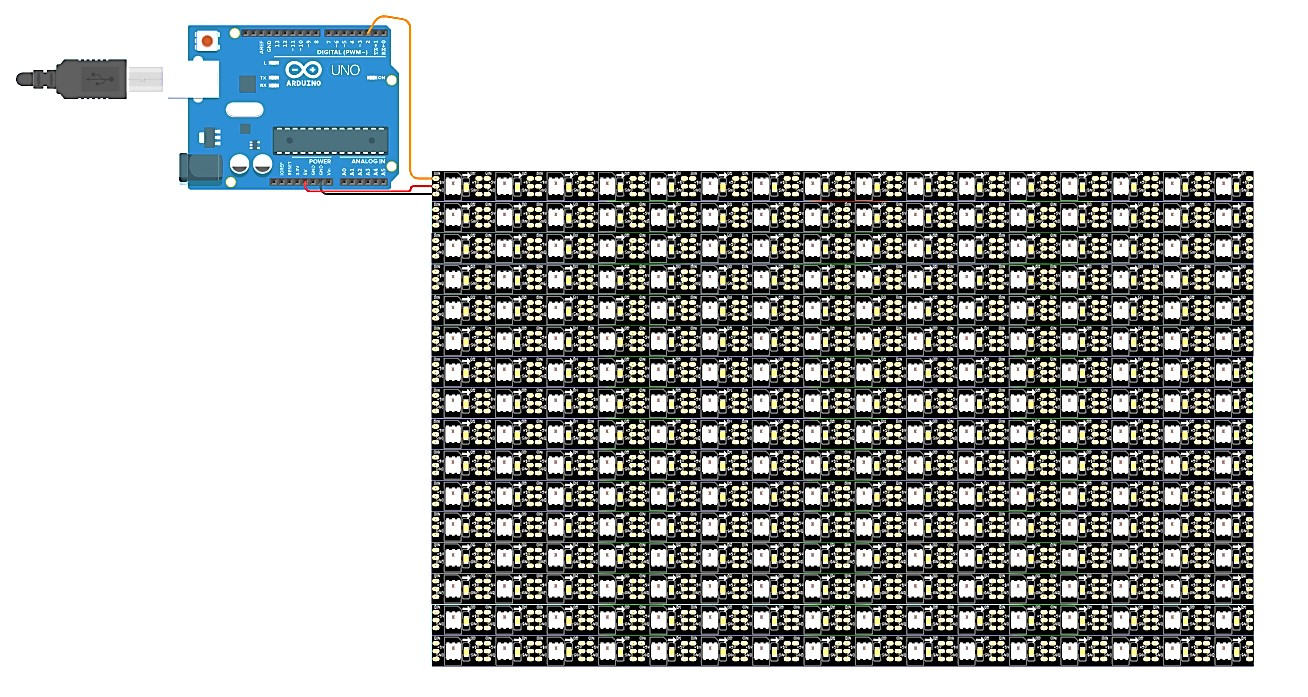
\includegraphics[width=13cm]{montaje.jpg}
\centering
\caption{Montaje}
\label{fig:Montaje}
\end{figure}

En el código de tinkercar, se recorre el arreglo, obteniendo las intensidades de rojo, verde y azul, los cuales se representan en cada led. Se observó un inconveniente en tinkercad cuando la intensidad de las tres componentes era la misma, por lo que se decidió variar un poco la intensidad de alguna componente cuando este fuese el caso.

\begin{lstlisting}[language=C++, label=tinker]
#include <Adafruit_NeoPixel.h>
#define LED_PIN    2
#define LED_COUNT  256
Adafruit_NeoPixel leds(LED_COUNT, LED_PIN, NEO_GRB+ 
 NEO_KHZ800);
byte array[3][16][16]={};
int fila=0;
int columna=0;
void setup()
{
  leds.begin();
  for (int i=0;i<LED_COUNT;i++){
    if(array[0][fila][columna]==array[1][fila][columna]
     && array[1][fila][columna]==array[2][fila][columna]){
      if(array[0][fila][columna]!=0)leds.setPixelColor(i,
       array[0][fila][columna], array[1][fila][columna],
        array[2][fila][columna]-1);
      else leds.setPixelColor(i, array[0][fila][columna],
       array[1][fila][columna],array[2][fila][columna]+1);
    }
  	else leds.setPixelColor(i, array[0][fila][columna],
  	 array[1][fila][columna],array[2][fila][columna]);
    if (columna==15){
    	columna=-1;
        fila++;
    }
  	columna++;
  }
  leds.show();
}
void loop(){}

\end{lstlisting}

\section{Resultados}\label{resultados}
\subsection{Submuestreo}
En la Figura (\ref{fig:CoreaS}), se presenta la bandera de Corea del Sur, cuyas dimensiones son 600x400, mientras que en la figura (\ref{fig:CoreaSled}), se presenta su representación en matrices led 16x16

\subsection{Sobremuestreo}
En la Figura (\ref{fig:Colombia}), se presenta la bandera de Colombia, cuyas dimensiones son 12x8, esta se encuentra ampliada en la presentación de este informe, sin embargo, se utilizaron sus dimensiones originales para el procesamiento. En la figura (\ref{fig:Colombialed}) se presenta la representación en matriz led, con variacions respecto al color de la bandera original de Colombia.
\begin{figure}[h]

\includegraphics[width=9cm]{CoreaS.jpg}
\centering
\caption{Bandera Corea del Sur 600x400}
\label{fig:CoreaS}
\end{figure}
\begin{figure}[h]
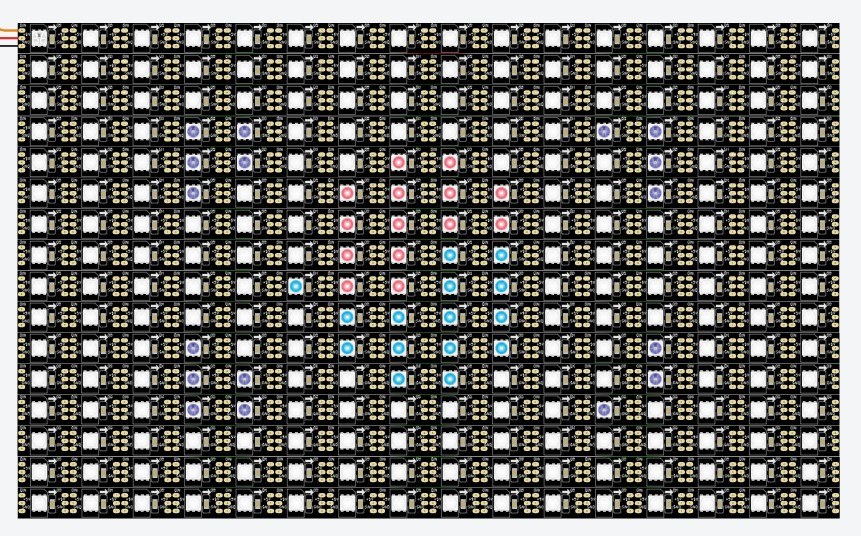
\includegraphics[width=9cm]{LedCoreaS.jpg}
\centering
\caption{Bandera Corea del Sur matriz led 16x16}
\label{fig:CoreaSled}
\end{figure}

\begin{figure}[h]

\includegraphics[width=3cm]{Col.jpg}
\centering
\caption{Bandera Colombia 12x8 pixeles (ampliada)}
\label{fig:Colombia}
\end{figure}

\begin{figure}[h]
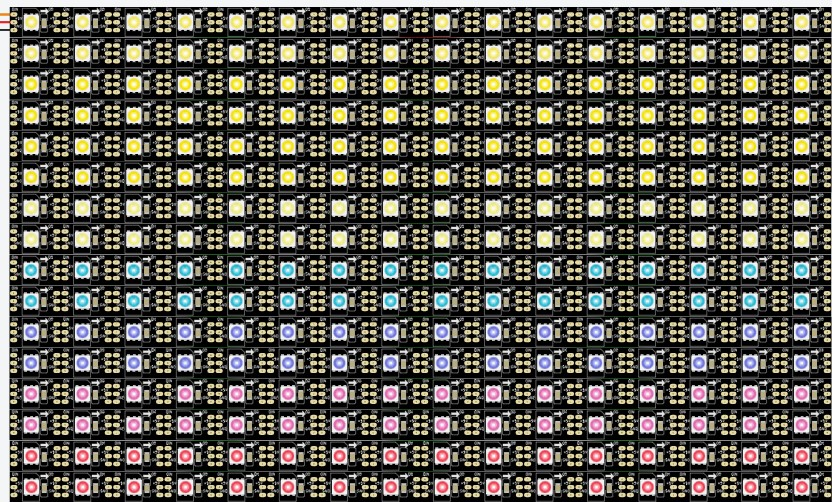
\includegraphics[width=8cm]{colled.jpg}
\centering
\caption{Bandera Colombia sobremuestreada matriz led 16x16}
\label{fig:Colombialed}
\end{figure}

\section{Conclusiones}
Durante la implementación del algoritmo de muestreo, se tenía la dificultad de dar una buena representación de la imagen, la cual fuese además simétrica, por lo que muestrear cada cuadrante de forma individual desde el centro de la imagen, permite solucionar este problema y facilita la observación de la imagen empleando el muestreo espacial.

Inicialmente se consideró que se estaba teniendo problemas en el sobremuestreo de las imágenes, pues en estas, el color de la bandera no quedaba como debería, sin embargo, al observar la imagen original que se quería sobremuestrear, se llegó a la conclusión de que esta representación estaba quedando de la manera adecuada, pues en las imágenes se ve una difuminación de los colores debido a la calidad o resolución espacial de la misma, por lo que el programa está recogiendo exactamente la intensidad de los pixeles que hay en la imagen, incluso si estos colores no hacen parte de los colores de la bandera original.

Con el desarrollo del parcial, se evidencia que es posible resolver problemáticas de la vida cotidiana con los conocimientos adquiridos en la programación con c++, específicamente en la programación orientada a objetos, en conjunto con la integración de microcontroladores como Arduino.

\end{document}
